\chapter{Smart contract implementation}\label{ch:implementation}
In the previous chapter the protocol was explained, some issues are identified, and mitigation strategies are proposed for the most critical ones.
This chapter describes how the entire protocol is implemented.
The development environment is made of Solidity on Ethereum~\cite{ethereum} and Hardhat as the development and testing framework.
In addition, the chapter also describes how \texttt{PrivacyFirstContract} and its extension, \texttt{PrivacySecondContract} interacts and which functions are overridden and the motivation behind every choice.

\section{Architecture}\label{sec:implementation-architecture}
The architecture is divided between on-chain operations and off chain ones, this distinction exists
because a lot of actions are not executable on the blockchain, like IPFS upload/download and ciphers
usage are not permitted on smart contacts due to the non-deterministic nature of operations such as encryption~\cite{wood2014ethereum}.
The off-chain operations are encapsulated in a SDK that allows actors to interact with the protocol without dealing directly with blockchain primitives.
The structure is composed by two contracts: the base protocol inspired to~\cite{bedogni2024crowdsensing} and another one that extends the base protocol with the mechanisms proposed in Section~\ref{sec:addressing-issues}.

\subsection{Contract hierarchy}\label{subsec:implementation-contract-hierarchy}
The \texttt{PrivacySecondContract} extends \texttt{PrivacyFirstContract}, reusing its core logic without modification.
The functionalities not covered by Section~\ref{sec:addressing-issues}, such as sender enrollment, bond system, majority consensus, and lifecycle are inherited without modification.
An overview of functions and more representative fields are shown in Figure~\ref{fig:proto-implementation-contract-hierarchy}.
\begin{figure}
    \begin{center}
        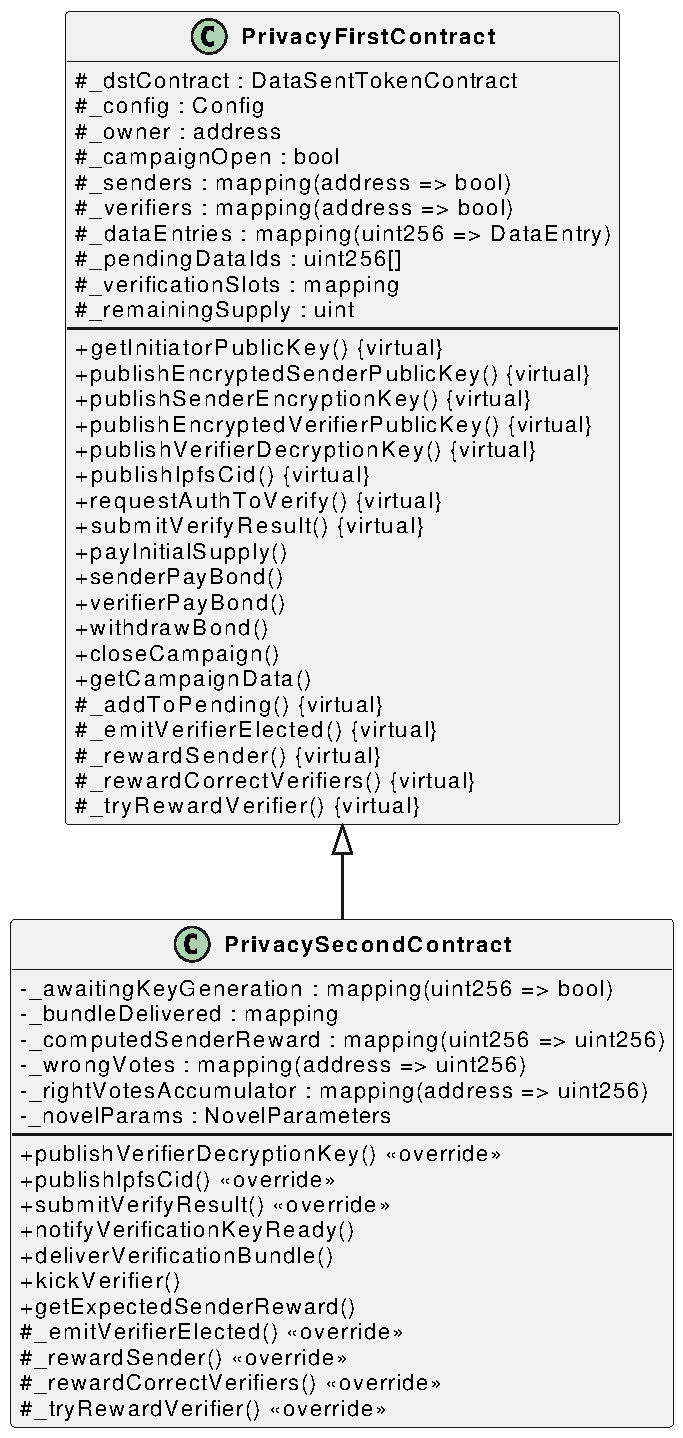
\includegraphics[width=0.50\textwidth]{diagrams/proto-implementation-contract-hierarchy-out}
        \caption{Class hierarchy of the two smart contracts}\label{fig:proto-implementation-contract-hierarchy}
    \end{center}\label{fig:proto-implementation-contract-hierarchy-container}
\end{figure}

There are four \texttt{internal} functions that have been overridden in the \texttt{PrivacySecondContract} to adapt them to the contract needs.

Since the extended contract needs to delivery verification bundles, to prevent duplicate delivery, a \texttt{\_bundleDelivered} mapping is introduced.
For this reason, once the bundle is sent the function \texttt{\_emitVerifierElected} is overridden in \texttt{PrivacySecondContract} to reset the delivery state, allowing a new bundle to be delivered if the verifier slot is reassigned.
This allows the usage of the same location of memory, the delivery of verification bundles is required in order to address the issue of verifiers trust, described in Section~\ref{subsec:addressing-issues-trusted-verifier-issue}.

Since in the Section~\ref{subsec:addressing-issues-geographical-incentive-issue} is described a mechanism to incentive data sensing in heterogeneous geographical areas, it is necessary to change the rewarding system.
For this reason, the method \texttt{\_rewardSender} is overridden and the only modification made is change the calculation of total payout.
In the first version of the contract, the reward is always the full base payout, in the novel one, the contract reads the pre-computed reward from storage.
The effective payout is calculated at the CID publish time, the contract execute the calculus in the \texttt{\_computeDecayedReward} function.
That function executes $k$ times the sqrt of a value (as shown in equation~\ref{eq:proto-design-reward-determination}), in \textit{O(log n)} time using the babylonian method~\cite{kosheleva2009babylonian}, to execute this operation, all values are scaled by a factor of \texttt{1E18} since the EVM, as noted in Section~\ref{sec:chunking-system}, is unable to execute floating point calculus.

The problem of missing verifiers penalties, in addition to bond loss, is discussed in Section~\ref{subsec:addressing-issues-missing-verifier-penalties}.
To address this issue, is required to modify how the smart contract collects the verifiers responses.
For this reason, the functions \texttt{\_rewardCorrectVerifiers} and \texttt{\_tryRewardVerifier} are modified and the responses are saved in mappings that keeps the count of correct votes and wrong ones.
These mappings are required to enforce the kick of systematically wrong voters, as proposed in Section~\ref{subsec:addressing-issues-missing-verifier-penalties}.

The \texttt{PrivacySecondContract} overrides also public functions; the function used to publish decryption key (\texttt{publishVerifierDecryptionKey}) in the \texttt{PrivacyFirstContract} publishes the decryption key through the VerifierEnrolled event, using a key shared among all enrolled verifiers.
In the novel contract, the function is overridden and publish the same event without the key, because, in order to avoid a single decryption key shared among all the verifiers, like described in~\ref{subsec:addressing-issues-trusted-verifier-issue}.
For these reasons, the function \texttt{publishIpfsCid}, is overridden and instead of adding the data in the pending data structure, the data entry requires that \texttt{B} to generate a per-data key pair ($KD_{enc}$, $KD_{dec}$), after which, \texttt{B} calls \texttt{notifyVerificationKeyReady} and the smart contract adds the data to pending data structure.
The novel event \texttt{VerifierElectedForData} notifies \texttt{B} that a verifier has been elected, upon which \texttt{B} delivers a verification bundle via \texttt{deliverVerificationBundle}.
Then a \texttt{VerifierVerificationBundleReady} is emitted and the verifier can finally calculate and submit the verification result using \texttt{submitVerifyResult} overridden function that checks the verification bundle delivery.

In addition, two new functions are introduced: \texttt{getExpectedSenderReward} and \texttt{kickVerifier}, the first one is informative and useful for users to understand which payout they will receive if they send data for a specific chunk in that moment.
The second one can be used from by campaign initiator \texttt{B} to exclude a verifier from the crowdsensing campaign.
In this case the verifier's bond is returned, as the exclusion from the campaign already constitutes a sufficient penalty, consistently with the design choice described in Section~\ref{subsec:addressing-issues-missing-verifier-penalties}.

A description of all overridden functions between the contracts is shown in Table~\ref{tab:contract-implementation-hierarchy-overrides}

\begin{table}
    \centering
    \begin{tabular}{|p{4cm}|p{3.5cm}|p{3.5cm}|p{2.5cm}|}
        \hline
        \textbf{Function} & \textbf{PFC} & \textbf{PSC} & \textbf{Reason} \\
        \hline
        {\texttt{publishVerifier-\newline DecryptionKey}}
        & Publishes decryption key on-chain via \texttt{VerifierEnrolled}
        & Emits \texttt{VerifierEnrolled} without key; key is generated off-chain
        & Trusted verifier flow (\ref{subsec:addressing-issues-trusted-verifier-issue}) \\
        \hline
        \texttt{publishIpfsCid}
        & Adds data to pending; reward is fixed base payout
        & Stores data awaiting key generation; computes decayed reward
        & Trusted verifier flow and reward decay (\ref{subsec:addressing-issues-trusted-verifier-issue},~\ref{subsec:addressing-issues-geographical-incentive-issue}) \\
        \hline
        \texttt{submitVerifyResult}
        & No prerequisite on bundle delivery
        & Requires \texttt{deliver-\newline Verification-\newline Bundle} to be called first
        & Trusted verifier flow (\ref{subsec:addressing-issues-trusted-verifier-issue}) \\
        \hline
        \texttt{\_emitVerifier-\newline Elected}
        & Emits election event and assigns slot
        & Additionally resets \texttt{\_bundle-\newline Delivered} flag
        & Allows bundle re-delivery on slot reassignment \\
        \hline
        \texttt{\_rewardSender}
        & Pays fixed base payout
        & Reads pre-computed reward from \newline \texttt{\_computedSender-\newline Reward}
        & Reward decay (\ref{subsec:addressing-issues-geographical-incentive-issue}) \\
        \hline
        \texttt{\_rewardCorrect-\newline Verifiers} \newline \texttt{\_tryRewardVerifier}
        & Distributes rewards based on majority
        & Additionally records correct and wrong votes per verifier
        & Verifier penalties (\ref{subsec:addressing-issues-missing-verifier-penalties}) \\
        \hline
    \end{tabular}
    \caption{Overridden functions between \texttt{PrivacyFirstContract} (PFC) and \texttt{PrivacySecondContract} (PSC)}
    \label{tab:contract-implementation-hierarchy-overrides}
\end{table}


\subsection{SDK layer}\label{subsec:implementation-sdk-layer}
TO BE EVALUATED
\section{Protocol phases implementation}\label{sec:implementation-protocol-phases}
\subsection{Initialization and deployment}\label{subsec:implementation-protocol-init}
\subsection{Sender enrollment}\label{subsec:implementation-sender-enrollment}
\subsection{Verifier enrollment}\label{subsec:implementation-verifier-enrollment}
\subsection{Data submission}\label{subsec:implementation-data-submission}
\subsection{Verification workflow}\label{subsec:implementation-verification}
\subsection{Extended protocol}\label{subsec:implementation-extended-protocol}
\section{Economic model}\label{sec:implementation-economic-model}
\subsection{DST token integration}\label{subsec:implementation-dst-integration}
\subsection{Reward logic}\label{subsec:implementation-reward}
\subsection{Bond logic}\label{subsec:implementation-bond}
\section{Gas optimization}\label{sec:implementation-gas-optimization}
\section{Contract lifecycle and state transitions}\label{sec:implementation-lifecycle}
TO BE EVALUATED